\documentclass[aspectratio=169]{beamer}

%
% Common preamble for all three parts.
%

%\usepackage[english]{babel}
% Turkce karakterler icin.
\usepackage[turkish,shorthands=:!]{babel}
\usepackage[utf8]{inputenc} % Kullanılan encodinge göre utf8 yerine latin5 de yazılabilir.
\usepackage[T1]{fontenc}

\usepackage{amsmath}
\usepackage{color}
\usepackage{minted}
\usepackage{hyperref}
\usepackage{multicol}
\usepackage{tabularx}
\usepackage{tikz}

% only inline todonotes work
\usepackage{xkeyval}
\usepackage[textsize=small]{todonotes}
\presetkeys{todonotes}{inline}{}

\usetikzlibrary{shapes,arrows,positioning,shadows}

% no nav buttons
\usenavigationsymbolstemplate{}

\newcommand{\bftt}[1]{\textbf{\texttt{#1}}}
\newcommand{\comment}[1]{{\color[HTML]{008080}\textit{\textbf{\texttt{#1}}}}}
\newcommand{\cmd}[1]{{\color[HTML]{008000}\bftt{#1}}}
\newcommand{\bs}{\char`\\}
\newcommand{\cmdbs}[1]{\cmd{\bs#1}}
\newcommand{\lcb}{\char '173}
\newcommand{\rcb}{\char '175}
\newcommand{\cmdbegin}[1]{\cmdbs{begin\lcb}\bftt{#1}\cmd{\rcb}}
\newcommand{\cmdend}[1]{\cmdbs{end\lcb}\bftt{#1}\cmd{\rcb}}

\newcommand{\wllogo}{\textbf{Overleaf}}

% this is where the example source files are loaded from
% do not include a trailing slash
\newcommand{\fileuri}{https://raw.github.com/jdleesmiller/latex-course/master/en}

\newcommand{\wlserver}{https://www.overleaf.com}
\newcommand{\wlnewdoc}[1]{\wlserver/docs?snip\_uri=\fileuri/#1\&splash=none}

\def\tikzname{Ti\emph{k}Z}

% from http://tex.stackexchange.com/questions/5226/keyboard-font-for-latex
\newcommand*\keystroke[1]{%
  \tikz[baseline=(key.base)]
    \node[%
      draw,
      fill=white,
      drop shadow={shadow xshift=0.25ex,shadow yshift=-0.25ex,fill=black,opacity=0.75},
      rectangle,
      rounded corners=2pt,
      inner sep=1pt,
      line width=0.5pt,
      font=\scriptsize\sffamily
    ](key) {#1\strut}
  ;
}
\newcommand{\keystrokebftt}[1]{\keystroke{\bftt{#1}}}

% stolen from minted.dtx
\newenvironment{exampletwoup}
  {\VerbatimEnvironment
   \begin{VerbatimOut}{example.out}}
  {\end{VerbatimOut}
   \setlength{\parindent}{0pt}
   \fbox{\begin{tabular}{l|l}
   \begin{minipage}{0.55\linewidth}
     \inputminted[fontsize=\small,resetmargins]{latex}{example.out}
   \end{minipage} &
   \begin{minipage}{0.35\linewidth}
     \input{example.out}
   \end{minipage}
   \end{tabular}}}

\newenvironment{exampletwouptiny}
  {\VerbatimEnvironment
   \begin{VerbatimOut}{example.out}}
  {\end{VerbatimOut}
   \setlength{\parindent}{0pt}
   \fbox{\begin{tabular}{l|l}
   \begin{minipage}{0.55\linewidth}
     \inputminted[fontsize=\scriptsize,resetmargins]{latex}{example.out}
   \end{minipage} &
   \begin{minipage}{0.35\linewidth}
     \setlength{\parskip}{6pt plus 1pt minus 1pt}%
     \raggedright\scriptsize\input{example.out}
   \end{minipage}
   \end{tabular}}}

\newenvironment{exampletwouptinynoframe}
  {\VerbatimEnvironment
   \begin{VerbatimOut}{example.out}}
  {\end{VerbatimOut}
   \setlength{\parindent}{0pt}
   \begin{tabular}{l|l}
   \begin{minipage}{0.55\linewidth}
     \inputminted[fontsize=\scriptsize,resetmargins]{latex}{example.out}
   \end{minipage} &
   \begin{minipage}{0.35\linewidth}
     \setlength{\parskip}{6pt plus 1pt minus 1pt}%
     \raggedright\scriptsize\input{example.out}
   \end{minipage}
   \end{tabular}}

\title{\LaTeX'e Etkileşimli Bir Giriş}
\author{Dr John D. Lees-Miller\\ Çeviri: Şevket Umut ÇAKIR(Pamukkale Üniversitesi)}
\titlegraphic{%

\includegraphics[height=36pt]{overleaf}\\[1em]

\includegraphics[height=24pt]{UoB-logo}
}


\subtitle{Bölüm 3: Sadece Makaleler Değil: Sunumlar \& Daha Fazlası}

\newcommand{\alice}[1]{\todo[color=green!40]{#1}}
\newcommand{\bob}[1]{\todo[color=purple!40]{#1}}

\begin{document}

%%%%%%%%%%%%%%%%%%%%%%%%%%%%%%%%%%%%%%%%%%%%%%%%%%%%%%%%%%%%%%%%%%%%%%%%%%%%%%%
%%%%%%%%%%%%%%%%%%%%%%%%%%%%%%%%%%%%%%%%%%%%%%%%%%%%%%%%%%%%%%%%%%%%%%%%%%%%%%%
%%%%%%%%%%%%%%%%%%%%%%%%%%%%%%%%%%%%%%%%%%%%%%%%%%%%%%%%%%%%%%%%%%%%%%%%%%%%%%%
\begin{frame}
\titlepage
\end{frame}

%%%%%%%%%%%%%%%%%%%%%%%%%%%%%%%%%%%%%%%%%%%%%%%%%%%%%%%%%%%%%%%%%%%%%%%%%%%%%%%
%%%%%%%%%%%%%%%%%%%%%%%%%%%%%%%%%%%%%%%%%%%%%%%%%%%%%%%%%%%%%%%%%%%%%%%%%%%%%%%
%%%%%%%%%%%%%%%%%%%%%%%%%%%%%%%%%%%%%%%%%%%%%%%%%%%%%%%%%%%%%%%%%%%%%%%%%%%%%%%
%\begin{frame}{Setup}
%\begin{itemize}
%\item Go to this URL in Google Chrome (\emph{not} Internet Explorer) to open
%these slides on your computer:
%\vskip 2em
%\begin{center}
%\fbox{\url{http://bit.ly/12WWWqj}}
%\end{center}
%\vskip 2em
%\item Here are the slides from the previous tutorial, for reference:
%\begin{center}
%\vskip 1em
%\fbox{\href{https://dl.dropboxusercontent.com/u/31383671/site/latex_course_v2/part1.pdf}{Part 1: The Basics}}
%\vskip 1em
%\fbox{\href{https://dl.dropboxusercontent.com/u/31383671/site/latex_course_v2/part2.pdf}{Part 2: Structured Documents \& More}}
%\end{center}
%\end{itemize}
%\end{frame}

%%%%%%%%%%%%%%%%%%%%%%%%%%%%%%%%%%%%%%%%%%%%%%%%%%%%%%%%%%%%%%%%%%%%%%%%%%%%%%%
%%%%%%%%%%%%%%%%%%%%%%%%%%%%%%%%%%%%%%%%%%%%%%%%%%%%%%%%%%%%%%%%%%%%%%%%%%%%%%%
%%%%%%%%%%%%%%%%%%%%%%%%%%%%%%%%%%%%%%%%%%%%%%%%%%%%%%%%%%%%%%%%%%%%%%%%%%%%%%%
\section{\LaTeX{} Özeti}

%%%%%%%%%%%%%%%%%%%%%%%%%%%%%%%%%%%%%%%%%%%%%%%%%%%%%%%%%%%%%%%%%%%%%%%%%%%%%%%
%%%%%%%%%%%%%%%%%%%%%%%%%%%%%%%%%%%%%%%%%%%%%%%%%%%%%%%%%%%%%%%%%%%%%%%%%%%%%%%
%%%%%%%%%%%%%%%%%%%%%%%%%%%%%%%%%%%%%%%%%%%%%%%%%%%%%%%%%%%%%%%%%%%%%%%%%%%%%%%
\begin{frame}[fragile]{\insertsection}
\begin{itemize}
	%\item You write your document in \texttt{plain text} with \cmd{commands} that describe its structure and meaning.
	%\item The \texttt{latex} program processes your text and commands to produce a beautifully formatted document.
	\item Dokümanınızı \texttt{düz metin} olarak \cmd{komutlarla} yazarsınız. Komutlar metnin yapısını ve anlamını tanımlar.
	\item \texttt{Latex} programı yazdığınız metin ve komutları işleyerek güzel biçimlendirilmiş dokümanlar üretir.
\end{itemize}
\vskip 2ex
\begin{center}
	%The rain in Spain falls \emph{mainly} on the plain.
	\begin{minted}[frame=single]{latex}
İspanya'da yağmur \emph{çoğunlukla} ovaya yağar.
	\end{minted}
	\vskip 2ex
	\tikz\node[single arrow,fill=gray,font=\ttfamily\bfseries,%
	rotate=270,xshift=-1em]{latex};
	\vskip 2ex
	\fbox{İspanya'da yağmur \emph{çoğunlukla} ovaya yağar.}
\end{center}
\end{frame}

%%%%%%%%%%%%%%%%%%%%%%%%%%%%%%%%%%%%%%%%%%%%%%%%%%%%%%%%%%%%%%%%%%%%%%%%%%%%%%%
%%%%%%%%%%%%%%%%%%%%%%%%%%%%%%%%%%%%%%%%%%%%%%%%%%%%%%%%%%%%%%%%%%%%%%%%%%%%%%%
%%%%%%%%%%%%%%%%%%%%%%%%%%%%%%%%%%%%%%%%%%%%%%%%%%%%%%%%%%%%%%%%%%%%%%%%%%%%%%%
\begin{frame}[fragile]{\insertsection: Komutlar \& Argümanlar}
\begin{itemize}
\item Bir komut \emph{ters eğik çizgi} \keystrokebftt{\bs} ile başlar.
\item Bazı komutlar süslü parantezler \keystrokebftt{\{} \keystrokebftt{\}} içinde bir \emph{argüman} alır.
\item Bazı komutlar da köşeli parantezler \keystrokebftt{[} \keystrokebftt{]} içinde  \emph{isteğe bağlı argümanlar} alır.
\vskip 2ex
\begin{exampletwouptiny}

\includegraphics[
  width=0.5\textwidth]{gerbil}


\includegraphics[
  width=0.3\textwidth,
  angle=270]{gerbil}
\end{exampletwouptiny}
\end{itemize}

\tiny{Görüntü lisansı: \href{https://pixabay.com/en/animal-apple-attractive-beautiful-1239390/}{CC0}}
\end{frame}

%%%%%%%%%%%%%%%%%%%%%%%%%%%%%%%%%%%%%%%%%%%%%%%%%%%%%%%%%%%%%%%%%%%%%%%%%%%%%%%
%%%%%%%%%%%%%%%%%%%%%%%%%%%%%%%%%%%%%%%%%%%%%%%%%%%%%%%%%%%%%%%%%%%%%%%%%%%%%%%
%%%%%%%%%%%%%%%%%%%%%%%%%%%%%%%%%%%%%%%%%%%%%%%%%%%%%%%%%%%%%%%%%%%%%%%%%%%%%%%
\begin{frame}[fragile]{\insertsection: Ortamlar}
\begin{itemize}
%\item The \cmdbs{begin} and \cmdbs{end} commands are used to create many
%different environments --- contexts.
\item \cmdbs{begin} ve \cmdbs{end} komutları birçok farklı ortam --- bağlam oluşturmak için kullanılır.

%\item The \bftt{itemize} and \bftt{enumerate} environments make lists.
\item \bftt{itemize} ve \bftt{enumerate} ortamları listeler oluşturur.
\vskip 2ex
\begin{exampletwouptiny}
\begin{itemize} % madde imleri icin
\item Biscuits
\item Tea
\end{itemize}

\begin{enumerate} % sayilar icin
\item Biscuits
\item Tea
\end{enumerate}
\end{exampletwouptiny}

\end{itemize}
\end{frame}

%%%%%%%%%%%%%%%%%%%%%%%%%%%%%%%%%%%%%%%%%%%%%%%%%%%%%%%%%%%%%%%%%%%%%%%%%%%%%%%
%%%%%%%%%%%%%%%%%%%%%%%%%%%%%%%%%%%%%%%%%%%%%%%%%%%%%%%%%%%%%%%%%%%%%%%%%%%%%%%
%%%%%%%%%%%%%%%%%%%%%%%%%%%%%%%%%%%%%%%%%%%%%%%%%%%%%%%%%%%%%%%%%%%%%%%%%%%%%%%
\begin{frame}[fragile]{\insertsection: Mathematics}
\begin{itemize}
\item \bftt{equation} ortamı numaralandırılmış denklemler oluşturur.
\begin{exampletwouptiny}
\begin{equation}
  \sum_{k=1}^{n} \frac{1}{2^k}
\end{equation}
\end{exampletwouptiny}
\vskip 2ex

\item Metnin içinde matematik sembolleri yazmak için dolar işareti \keystrokebftt{\$} kullanın.\\[1ex]
\begin{exampletwouptiny}
% iyi degil:
a ve b iki ayri pozitif tamsayi olsun
ve c = a - b + 1 olsun.

% daha iyi:
$a$ ve $b$ iki ayri pozitif tamsayi 
ve $c = a - b + 1$ olsun.
\end{exampletwouptiny}
\vskip 2ex
\item Dolar işaretlerini her zaman çift olarak kullanın --- bir tanesi matematik ifadesini başlatmak için, diğeri bitirmek için.
\vskip 1em
{\scriptsize Aslında, \bftt{\$...\$}  ifadesini 
\cmdbegin{math}\bftt{...}\cmdend{math} şeklinde yazabilirdik.}
\end{itemize}
\end{frame}

%%%%%%%%%%%%%%%%%%%%%%%%%%%%%%%%%%%%%%%%%%%%%%%%%%%%%%%%%%%%%%%%%%%%%%%%%%%%%%%
%%%%%%%%%%%%%%%%%%%%%%%%%%%%%%%%%%%%%%%%%%%%%%%%%%%%%%%%%%%%%%%%%%%%%%%%%%%%%%%
%%%%%%%%%%%%%%%%%%%%%%%%%%%%%%%%%%%%%%%%%%%%%%%%%%%%%%%%%%%%%%%%%%%%%%%%%%%%%%%
\begin{frame}[fragile]{\insertsection: Belge Yapısı}
\begin{itemize}{\small
\item \cmdbs{documentclass} ile başlar --- ne tür bir belge.
\item Meta veriler (\cmdbs{title} and \cmdbs{author}) ve paketler başlangıçta yer alır.
\item İçerik \cmdbegin{document} ve \cmdend{document} arasındadır.
\item \cmdbs{maketitle} komutu başlığı oluşturur ; \cmdbs{section} komutu numaralandırılmış bölümleri oluşturur.
}\end{itemize}
\begin{minipage}{0.55\linewidth}
\inputminted[fontsize=\scriptsize,frame=single,resetmargins]{latex}%
  {recap-structure.tex}
\end{minipage}
\begin{minipage}{0.35\linewidth}
% trim: l b r t

\includegraphics[width=\textwidth,clip,trim=1.5in 7in 3in 2in]{recap-structure.pdf}
\end{minipage}
\end{frame}

%%%%%%%%%%%%%%%%%%%%%%%%%%%%%%%%%%%%%%%%%%%%%%%%%%%%%%%%%%%%%%%%%%%%%%%%%%%%%%%
%%%%%%%%%%%%%%%%%%%%%%%%%%%%%%%%%%%%%%%%%%%%%%%%%%%%%%%%%%%%%%%%%%%%%%%%%%%%%%%
%%%%%%%%%%%%%%%%%%%%%%%%%%%%%%%%%%%%%%%%%%%%%%%%%%%%%%%%%%%%%%%%%%%%%%%%%%%%%%%
\begin{frame}[fragile]{\insertsection: Alıştırma}

\begin{enumerate}
\item Kısa bir makale için metin:\footnote{\url{http://www.cgd.ucar.edu/cms/agu/scientific_talk.html} sitesinden}
\begin{center}
\fbox{\href{\wlnewdoc{recap-exercise.tex}}{%
Alıştırmayı  \wllogo{}'te açmak için tıklayın}}
\end{center}
\vskip 2ex
\item Metnin aşağıdaki gibi görünmesi için \LaTeX{} komutları ekleyin:
\begin{center}
\fbox{\href{\fileuri/recap-exercise-solution.pdf} yazmak için, \emph{kaçış} karakteri olarak ters bölü sembolü ile birlikte kullanın (\cmdbs{\%}).
\item Denklemi oluştururken, bölme işlemi için \cmdbs{frac} ve parantezler için  \cmdbs{left(} ve \cmdbs{right)} kullanın.
\end{itemize}
\end{block}
\end{frame}

%%%%%%%%%%%%%%%%%%%%%%%%%%%%%%%%%%%%%%%%%%%%%%%%%%%%%%%%%%%%%%%%%%%%%%%%%%%%%%%
%%%%%%%%%%%%%%%%%%%%%%%%%%%%%%%%%%%%%%%%%%%%%%%%%%%%%%%%%%%%%%%%%%%%%%%%%%%%%%%
%%%%%%%%%%%%%%%%%%%%%%%%%%%%%%%%%%%%%%%%%%%%%%%%%%%%%%%%%%%%%%%%%%%%%%%%%%%%%%%
\section{\protect\bftt{beamer} ile Sunumlar}

%%%%%%%%%%%%%%%%%%%%%%%%%%%%%%%%%%%%%%%%%%%%%%%%%%%%%%%%%%%%%%%%%%%%%%%%%%%%%%%
%%%%%%%%%%%%%%%%%%%%%%%%%%%%%%%%%%%%%%%%%%%%%%%%%%%%%%%%%%%%%%%%%%%%%%%%%%%%%%%
%%%%%%%%%%%%%%%%%%%%%%%%%%%%%%%%%%%%%%%%%%%%%%%%%%%%%%%%%%%%%%%%%%%%%%%%%%%%%%%
\begin{frame}[fragile]{\insertsection}
\begin{itemize}
\item Beamer, \LaTeX{}'de sunumlar oluşturmak için bir paket(bunun gibi!).
\item \bftt{beamer} belge sınıfını sağlar.
\item Slaytlar oluşturmak için \bftt{frame} ortamını kullanın.
\end{itemize}
\begin{minipage}{0.55\linewidth}
\inputminted[fontsize=\scriptsize,frame=single,resetmargins]{latex}%
  {beamer-minimal.tex}
\end{minipage}
\begin{minipage}{0.35\linewidth}
% trim: l b r t
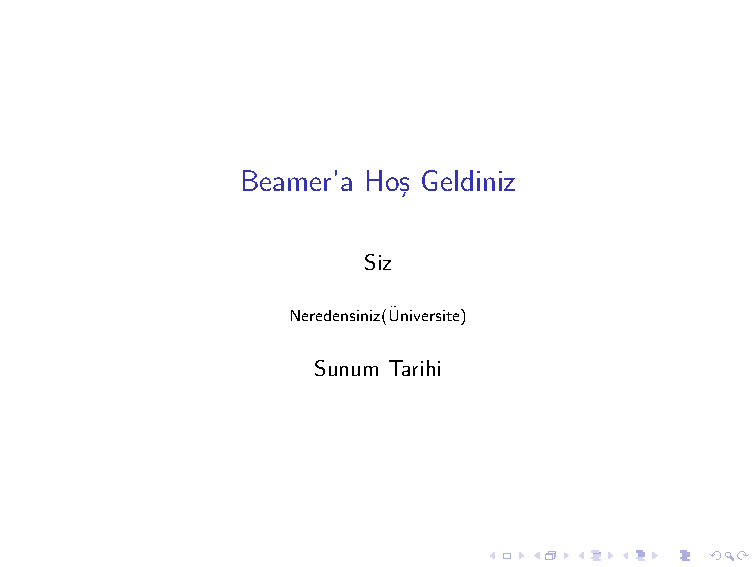
\includegraphics[width=\textwidth,clip,trim=1in 1in 1in 1in]{beamer-minimal.pdf}
\end{minipage}
\end{frame}

%%%%%%%%%%%%%%%%%%%%%%%%%%%%%%%%%%%%%%%%%%%%%%%%%%%%%%%%%%%%%%%%%%%%%%%%%%%%%%%
%%%%%%%%%%%%%%%%%%%%%%%%%%%%%%%%%%%%%%%%%%%%%%%%%%%%%%%%%%%%%%%%%%%%%%%%%%%%%%%
%%%%%%%%%%%%%%%%%%%%%%%%%%%%%%%%%%%%%%%%%%%%%%%%%%%%%%%%%%%%%%%%%%%%%%%%%%%%%%%
\begin{frame}[fragile]{\insertsection: Birlikte Takip Edin}

\begin{itemize}
\item Aşağıdaki slaytlarda ilerlerken, \wllogo{}'teki örnek belgeye yazarak örnekleri deneyin.

\end{itemize}
\vskip 2ex
\begin{center}
\fbox{\href{\wlnewdoc{beamer-minimal.tex}}{%
Örnek belgeyi \wllogo{}'te açmak için tıklayın}}
\end{center}
\end{frame}

%%%%%%%%%%%%%%%%%%%%%%%%%%%%%%%%%%%%%%%%%%%%%%%%%%%%%%%%%%%%%%%%%%%%%%%%%%%%%%%
%%%%%%%%%%%%%%%%%%%%%%%%%%%%%%%%%%%%%%%%%%%%%%%%%%%%%%%%%%%%%%%%%%%%%%%%%%%%%%%
%%%%%%%%%%%%%%%%%%%%%%%%%%%%%%%%%%%%%%%%%%%%%%%%%%%%%%%%%%%%%%%%%%%%%%%%%%%%%%%
\begin{frame}[fragile]
\frametitle{\insertsection: Çerçeveler}
\begin{itemize}
\item Sayfaya/Çerçeveye başlık vermek için \cmdbs{frametitle} kullanın.
\item Ardından çerçeveye içerik ekleyin.
\item Bu çerçevenin kaynağı şu şekildedir:
\vskip 2ex
\inputminted[fontsize=\scriptsize,frame=single,resetmargins,breaklines]{latex}%
  {beamer-frame.tex}
\end{itemize}
\end{frame}

%%%%%%%%%%%%%%%%%%%%%%%%%%%%%%%%%%%%%%%%%%%%%%%%%%%%%%%%%%%%%%%%%%%%%%%%%%%%%%%
%%%%%%%%%%%%%%%%%%%%%%%%%%%%%%%%%%%%%%%%%%%%%%%%%%%%%%%%%%%%%%%%%%%%%%%%%%%%%%%
%%%%%%%%%%%%%%%%%%%%%%%%%%%%%%%%%%%%%%%%%%%%%%%%%%%%%%%%%%%%%%%%%%%%%%%%%%%%%%%
\begin{frame}[fragile]{\insertsection: Sections}
\begin{itemize}
\item Çerçeveleri \cmdbs{frame} gruplamak için \cmdbs{section} kullanılabilir. \bftt{beamer} bölümleri kullanarak otomatik anahat oluşturur.
%\item You can use \cmdbs{section}s to group your \bftt{frame}s, and
%\bftt{beamer} will use them to create an automatic outline.
\item Anahat oluşturmak için \cmdbs{tableofcontents} komutunu kullanın. Bu sunum için burada var. \cmdbs{currentsection} özelliği mevcut bölümü vurgular.
%\item To generate an outline, use the \cmdbs{tableofcontents} command. Here's
%one for this presentation. The \bftt{currentsection} option highlights the current section.
\vskip 2ex
\begin{exampletwouptiny}
\tableofcontents[currentsection]
\end{exampletwouptiny}
\end{itemize}
\end{frame}

%%%%%%%%%%%%%%%%%%%%%%%%%%%%%%%%%%%%%%%%%%%%%%%%%%%%%%%%%%%%%%%%%%%%%%%%%%%%%%%
%%%%%%%%%%%%%%%%%%%%%%%%%%%%%%%%%%%%%%%%%%%%%%%%%%%%%%%%%%%%%%%%%%%%%%%%%%%%%%%
%%%%%%%%%%%%%%%%%%%%%%%%%%%%%%%%%%%%%%%%%%%%%%%%%%%%%%%%%%%%%%%%%%%%%%%%%%%%%%%
\begin{frame}[fragile]{\insertsection: Çoklu Sütunlar}
\begin{columns}
\begin{column}{0.4\textwidth}
\begin{itemize}
%\item Use the \bftt{columns} and \bftt{column} environments to break the slide into columns.
\item Slaytı sütunlara bölmek için \bftt{columns} ve \bftt{column} ortamlarını kullanın.
%\item The argument for each \bftt{column} determines its width.
\item Her sütun(\bftt{column}) için argüman genişliği belirler.
%\item See also the \bftt{multicol} package, which automatically breaks your content into columns.
\item İçeriğinizi otomatik olarak sütunlara bölen \bftt{multicol} paketine de bakın.
\end{itemize}
\end{column}
\begin{column}{0.6\textwidth}
\begin{minted}[fontsize=\scriptsize,frame=single]{latex}
\begin{columns}
  \begin{column}{0.4\textwidth}
    \begin{itemize}
    \item Slaytı sütulara ...
    \item Her sütun ...
    \item İçeriğinizi otomatik ...
    \end{itemize}
  \end{column}
  \begin{column}{0.6\textwidth}
    % ikinci sütun
  \end{column}
\end{columns}
\end{minted}
\end{column}
\end{columns}
\end{frame}

%%%%%%%%%%%%%%%%%%%%%%%%%%%%%%%%%%%%%%%%%%%%%%%%%%%%%%%%%%%%%%%%%%%%%%%%%%%%%%%
%%%%%%%%%%%%%%%%%%%%%%%%%%%%%%%%%%%%%%%%%%%%%%%%%%%%%%%%%%%%%%%%%%%%%%%%%%%%%%%
%%%%%%%%%%%%%%%%%%%%%%%%%%%%%%%%%%%%%%%%%%%%%%%%%%%%%%%%%%%%%%%%%%%%%%%%%%%%%%%
\begin{frame}[fragile]{\insertsection: Vurgular}
\begin{itemize}

\item Vurgu için \cmdbs{emph} ve \cmdbs{alert} kullanın:
\vskip 1ex
\begin{exampletwouptiny}
Bunun \alert{onemli} bir nokta
oldugunu \emph{belirtmeliyim}.
\end{exampletwouptiny}
\vskip 1ex

\item Kalın veya italik olarak belirtin:
\vskip 1ex
\begin{exampletwouptiny}
\textbf{Kalin} metin.
\textit{italik} metin.
\end{exampletwouptiny}
\vskip 1ex

\item Veya bir renk tanımlayın:
\vskip 1ex
\begin{exampletwouptiny}
\textcolor{red}{Durur}
ve \textcolor{green}{baslar}.
\end{exampletwouptiny}
\vskip 1ex
\item Daha fazla renk ve özel renkler için \url{http://www.math.umbc.edu/~rouben/beamer/quickstart-Z-H-25.html} adresine bakın.
\end{itemize}
\end{frame}

%%%%%%%%%%%%%%%%%%%%%%%%%%%%%%%%%%%%%%%%%%%%%%%%%%%%%%%%%%%%%%%%%%%%%%%%%%%%%%%
%%%%%%%%%%%%%%%%%%%%%%%%%%%%%%%%%%%%%%%%%%%%%%%%%%%%%%%%%%%%%%%%%%%%%%%%%%%%%%%
%%%%%%%%%%%%%%%%%%%%%%%%%%%%%%%%%%%%%%%%%%%%%%%%%%%%%%%%%%%%%%%%%%%%%%%%%%%%%%%
\begin{frame}[fragile]{\insertsection: Şekiller}
\begin{itemize}
\item \bftt{graphicx} paketinden \cmdbs{includegraphics} kullanın.
\item \bftt{figure} ortamı \bftt{beamer}'da varsayılan olarak ortalanır.
\vskip 2ex
\begin{exampletwouptiny}
\begin{figure}

\includegraphics[
  width=0.5\textwidth]{gerbil}
\end{figure}
\end{exampletwouptiny}
\end{itemize}

\tiny{Görüntü lisansı: \href{https://pixabay.com/en/animal-apple-attractive-beautiful-1239390/}{CC0}}
\end{frame}

%%%%%%%%%%%%%%%%%%%%%%%%%%%%%%%%%%%%%%%%%%%%%%%%%%%%%%%%%%%%%%%%%%%%%%%%%%%%%%%
%%%%%%%%%%%%%%%%%%%%%%%%%%%%%%%%%%%%%%%%%%%%%%%%%%%%%%%%%%%%%%%%%%%%%%%%%%%%%%%
%%%%%%%%%%%%%%%%%%%%%%%%%%%%%%%%%%%%%%%%%%%%%%%%%%%%%%%%%%%%%%%%%%%%%%%%%%%%%%%
\begin{frame}[fragile]{\insertsection: Tablolar}
\begin{itemize}
\item \LaTeX{} çindeki tablolara alışmak biraz zaman alır.
\item \bftt{tabularx} paketinden \bftt{tabular} ortamını kullanın.
\item Argüman sütun hizalamasını belirtir --- \textbf{l}eft, \textbf{r}ight, \textbf{r}ight.
%\item The argument specifies column alignment --- \textbf{l}eft, \textbf{r}ight, \textbf{r}ight.
\begin{exampletwouptiny}
\begin{tabular}{lrr}
Urun   & Adet & Fiyat \$ \\
Arac & 1   & 199.99  \\
Gerec & 2   & 399.99  \\
Kablo  & 3   & 19.99   \\
\end{tabular}
\end{exampletwouptiny}
\item Dikey çizgileri de belirtir; yatay çizgi için \cmdbs{hline} kullanın.
\begin{exampletwouptiny}
\begin{tabular}{|l|r|r|} \hline
Urun   & Adet & Fiyat \$ \\\hline
Arac & 1   & 199.99  \\
Gerec & 2   & 399.99  \\
Kablo  & 3   & 19.99   \\\hline
\end{tabular}
\end{exampletwouptiny}
\item Sütunları ayırmak için ampersand \keystrokebftt{\&} ve yeni satıra başlamak için çift ters eğik çizgi \keystrokebftt{\bs}\keystrokebftt{\bs} kullanın.
%\item Use an ampersand \keystrokebftt{\&} to separate columns and a double backslash \keystrokebftt{\bs}\keystrokebftt{\bs} to start a new row.
\end{itemize}
\end{frame}

%%%%%%%%%%%%%%%%%%%%%%%%%%%%%%%%%%%%%%%%%%%%%%%%%%%%%%%%%%%%%%%%%%%%%%%%%%%%%%%
%%%%%%%%%%%%%%%%%%%%%%%%%%%%%%%%%%%%%%%%%%%%%%%%%%%%%%%%%%%%%%%%%%%%%%%%%%%%%%%
%%%%%%%%%%%%%%%%%%%%%%%%%%%%%%%%%%%%%%%%%%%%%%%%%%%%%%%%%%%%%%%%%%%%%%%%%%%%%%%
\begin{frame}[fragile]{\insertsection: Bloklar}
\begin{itemize}
\item \bftt{block} ortamı başlıklı bir kutu oluşturur.
\begin{exampletwouptiny}
\begin{block}{Ilginc Gercek}
Bu onemli.
\end{block}

\begin{alertblock}{Egitici Oyku}
Bu gercekten onemli!
\end{alertblock}
\end{exampletwouptiny}

\item Tam olarak nasıl göründükleri temaya bağlıdır \ldots
\end{itemize}
\end{frame}

%%%%%%%%%%%%%%%%%%%%%%%%%%%%%%%%%%%%%%%%%%%%%%%%%%%%%%%%%%%%%%%%%%%%%%%%%%%%%%%
%%%%%%%%%%%%%%%%%%%%%%%%%%%%%%%%%%%%%%%%%%%%%%%%%%%%%%%%%%%%%%%%%%%%%%%%%%%%%%%
%%%%%%%%%%%%%%%%%%%%%%%%%%%%%%%%%%%%%%%%%%%%%%%%%%%%%%%%%%%%%%%%%%%%%%%%%%%%%%%
\begin{frame}[fragile]
\frametitle{\insertsection: Temalar}
\begin{itemize}
\item Temaları kullanarak sunumunuzun görünümünü özelleştirin.
\item Geniş bir tema koleksiyonu için \url{http://deic.uab.es/~iblanes/beamer_gallery/index_by_theme.html} adresine bakın.
\end{itemize}
\begin{minipage}{0.55\linewidth}
\inputminted[fontsize=\scriptsize,frame=single,resetmargins]{latex}%
  {beamer-theme.tex}
\end{minipage}
\begin{minipage}{0.35\linewidth}
% trim: l b r t
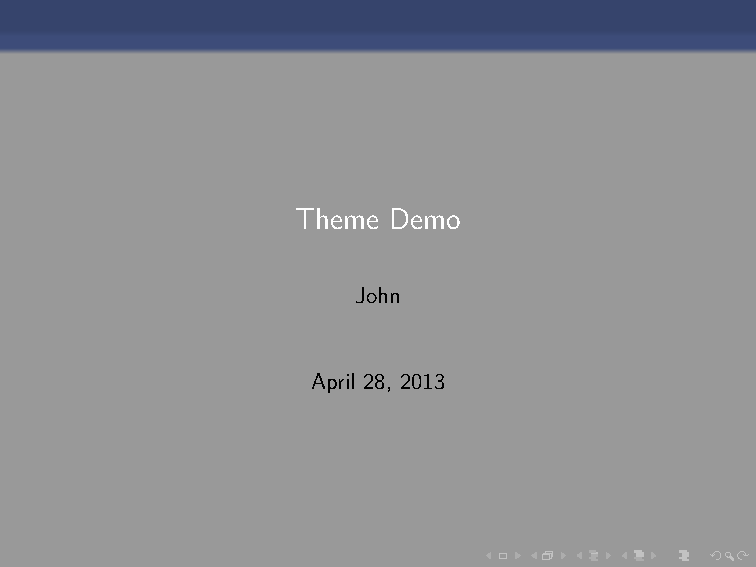
\includegraphics[width=\textwidth]{beamer-theme.pdf}
\end{minipage}
\end{frame}

%%%%%%%%%%%%%%%%%%%%%%%%%%%%%%%%%%%%%%%%%%%%%%%%%%%%%%%%%%%%%%%%%%%%%%%%%%%%%%%
%%%%%%%%%%%%%%%%%%%%%%%%%%%%%%%%%%%%%%%%%%%%%%%%%%%%%%%%%%%%%%%%%%%%%%%%%%%%%%%
%%%%%%%%%%%%%%%%%%%%%%%%%%%%%%%%%%%%%%%%%%%%%%%%%%%%%%%%%%%%%%%%%%%%%%%%%%%%%%%
\begin{frame}[fragile]{\insertsection: Animasyon}
\begin{itemize}
\item Bir çerçeve birden çok slayt oluşturabilir.
\item Bir slaytın yalnızca bir kısmını göstermek için \cmdbs{pause} komutunu kullanın.
\vskip 2ex
\begin{exampletwouptinynoframe}
\begin{itemize}
\item Beklentiyi 
\pause \item hissedebiliyor musun?
\end{itemize}
\end{exampletwouptinynoframe}
\vskip 2ex
\item \bftt{beamer} içinde animasyon oluşturmanın daha birçok akıllı yolu vardır; 
\cmdbs{only}, \cmdbs{alt}, ve \cmdbs{uncover} komutlarına da bakın.
%\item There many more clever ways of making animations in \bftt{beamer}; see
%also the \cmdbs{only}, \cmdbs{alt}, and \cmdbs{uncover} commands.
\end{itemize}
\end{frame}

%%%%%%%%%%%%%%%%%%%%%%%%%%%%%%%%%%%%%%%%%%%%%%%%%%%%%%%%%%%%%%%%%%%%%%%%%%%%%%%
%%%%%%%%%%%%%%%%%%%%%%%%%%%%%%%%%%%%%%%%%%%%%%%%%%%%%%%%%%%%%%%%%%%%%%%%%%%%%%%
%%%%%%%%%%%%%%%%%%%%%%%%%%%%%%%%%%%%%%%%%%%%%%%%%%%%%%%%%%%%%%%%%%%%%%%%%%%%%%%
\begin{frame}[fragile]{\insertsection: Alıştırma}

Peter Norvig'in mükemmel ``Gettysburg Powerpoint Sunumunu'' \bftt{beamer}'da yeniden oluşturun.\footnote{\url{http://norvig.com/Gettysburg}}

\begin{enumerate}
\item Bu alıştırmayı \wllogo{}'da açın:
\begin{center}
\fbox{\href{\wlnewdoc{beamer-exercise.tex}}{%
Bu alıştırmayı \wllogo{}'da açmak için tıklayın.}}
\end{center}
\vskip 2ex
\item Bu resmi bilgisayarınıza indirin ve dosyalar menüsünden \wllogo{}'a yükleyin.
\begin{center}
\fbox{\href{\fileuri/gettysburg_graph.png?dl=1}{Resmi indirmek için tıklayın}}
\end{center}
\vskip 2ex
\item Metne \LaTeX{} komutları ekleyerek metnin böyle görünmesini sağlayın:
\begin{center}
\fbox{\href{\fileuri/beamer-exercise-solution.pdf}{%
Model belgeyi açmak için tıklayın}}
\end{center}
\end{enumerate}
\end{frame}

%%%%%%%%%%%%%%%%%%%%%%%%%%%%%%%%%%%%%%%%%%%%%%%%%%%%%%%%%%%%%%%%%%%%%%%%%%%%%%%
%%%%%%%%%%%%%%%%%%%%%%%%%%%%%%%%%%%%%%%%%%%%%%%%%%%%%%%%%%%%%%%%%%%%%%%%%%%%%%%
%%%%%%%%%%%%%%%%%%%%%%%%%%%%%%%%%%%%%%%%%%%%%%%%%%%%%%%%%%%%%%%%%%%%%%%%%%%%%%%
\section{\protect\tikzname{} ile Çizimler}

%%%%%%%%%%%%%%%%%%%%%%%%%%%%%%%%%%%%%%%%%%%%%%%%%%%%%%%%%%%%%%%%%%%%%%%%%%%%%%%
%%%%%%%%%%%%%%%%%%%%%%%%%%%%%%%%%%%%%%%%%%%%%%%%%%%%%%%%%%%%%%%%%%%%%%%%%%%%%%%
%%%%%%%%%%%%%%%%%%%%%%%%%%%%%%%%%%%%%%%%%%%%%%%%%%%%%%%%%%%%%%%%%%%%%%%%%%%%%%%
\begin{frame}[fragile]{\insertsection}
\begin{itemize}
\item \tikzname{}, \LaTeX{}'te şekil çizmek için bir pakettir.
\item \LaTeX{} içinde güçlü bir çizim dili tanımlar. Kısa programlar şaşırtıcı derecede karmaşık şeyler çizebilir.
\begin{figure}
\href{http://www.texample.net/tikz/examples/rotated-triangle/}{%
  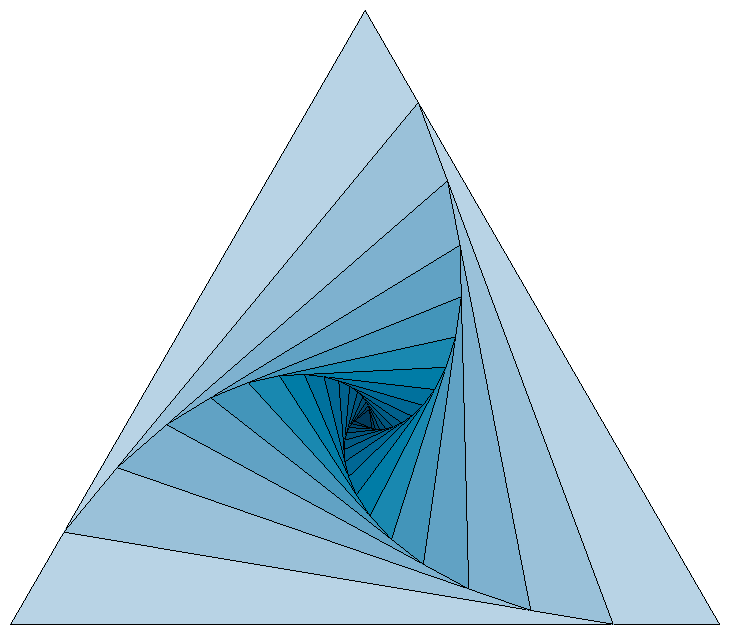
\includegraphics[width=0.35\textwidth]{rotated-triangle}}
\end{figure}
%\item We'll start with simple things. To draw a line in \tikzname:
\item Basit şeylerle başlayacağız. \tikzname'de bir çizgi çizmek için
\vskip 1ex
\begin{exampletwouptiny}
\begin{tikzpicture}
\draw (0,0) -- (1,1); % bir cizgi
\end{tikzpicture}
\end{exampletwouptiny}
\end{itemize}
\end{frame}

%%%%%%%%%%%%%%%%%%%%%%%%%%%%%%%%%%%%%%%%%%%%%%%%%%%%%%%%%%%%%%%%%%%%%%%%%%%%%%%
%%%%%%%%%%%%%%%%%%%%%%%%%%%%%%%%%%%%%%%%%%%%%%%%%%%%%%%%%%%%%%%%%%%%%%%%%%%%%%%
%%%%%%%%%%%%%%%%%%%%%%%%%%%%%%%%%%%%%%%%%%%%%%%%%%%%%%%%%%%%%%%%%%%%%%%%%%%%%%%
\begin{frame}[fragile]{\insertsection: Koordinatlar}
\begin{itemize}
\item Varsayılan koordinatlar, her zamanki anlamda santimetredir:
\begin{figure}
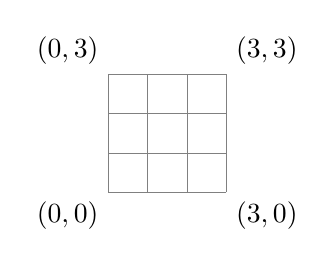
\begin{tikzpicture}[scale=0.5]
\draw[help lines] (0,0) grid (3,3);
\node[below left] at (0,0) {$(0,0)$};
\node[below right] at (3,0) {$(3,0)$};
\node[above right] at (3,3) {$(3,3)$};
\node[above left] at (0,3) {$(0,3)$};
\end{tikzpicture}
\end{figure}
\item \tikzname{} ile çalışırken bir ızgara çizmeye yardımcı olur:
\vskip 1ex
\begin{exampletwouptiny}

\begin{tikzpicture}
\draw[help lines] (0,0) grid (3,3);
\end{tikzpicture}
\end{exampletwouptiny}
\end{itemize}
\end{frame}

%%%%%%%%%%%%%%%%%%%%%%%%%%%%%%%%%%%%%%%%%%%%%%%%%%%%%%%%%%%%%%%%%%%%%%%%%%%%%%%
%%%%%%%%%%%%%%%%%%%%%%%%%%%%%%%%%%%%%%%%%%%%%%%%%%%%%%%%%%%%%%%%%%%%%%%%%%%%%%%
%%%%%%%%%%%%%%%%%%%%%%%%%%%%%%%%%%%%%%%%%%%%%%%%%%%%%%%%%%%%%%%%%%%%%%%%%%%%%%%
\begin{frame}[fragile]{\insertsection: Çizgiler}
\begin{itemize}
\item Ok uçları ve çizgi stilleri, \cmdbs{draw} komutuna argüman olarak verilir.
\item Her çizim komutunu bir noktalı virgül \keystrokebftt{;} ile bitirin.
\vskip 1ex
\begin{exampletwouptiny}
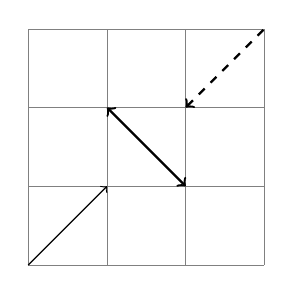
\begin{tikzpicture}
\draw[help lines] (0,0) grid (3,3);
\draw[->] (0,0) -- (1,1);
\draw[<->, thick] (2,1) -- (1,2);
\draw[<-, thick, dashed] (2,2)--(3,3);
\end{tikzpicture}
\end{exampletwouptiny}
\end{itemize}
\end{frame}

%%%%%%%%%%%%%%%%%%%%%%%%%%%%%%%%%%%%%%%%%%%%%%%%%%%%%%%%%%%%%%%%%%%%%%%%%%%%%%%
%%%%%%%%%%%%%%%%%%%%%%%%%%%%%%%%%%%%%%%%%%%%%%%%%%%%%%%%%%%%%%%%%%%%%%%%%%%%%%%
%%%%%%%%%%%%%%%%%%%%%%%%%%%%%%%%%%%%%%%%%%%%%%%%%%%%%%%%%%%%%%%%%%%%%%%%%%%%%%%
\begin{frame}[fragile]{\insertsection: Yollar}
\begin{itemize}
\item Bir yol oluşturmak için birden çok nokta belirtebilirsiniz.
\item Oklar yalnızca yolun sonunda görünecektir.
\vskip 1ex
\begin{exampletwouptiny}
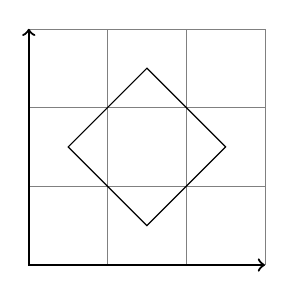
\begin{tikzpicture}
\draw[help lines] (0,0) grid (3,3);
% eksenler:
\draw[<->, thick] (0,3)--(0,0)--(3,0);
% baklava dilimi:
\draw (1.5,0.5) -- (2.5,1.5) -- 
      (1.5,2.5) -- (0.5,1.5) --
      cycle; % yolu kapat
\end{tikzpicture}
\end{exampletwouptiny}
\end{itemize}
\end{frame}

%%%%%%%%%%%%%%%%%%%%%%%%%%%%%%%%%%%%%%%%%%%%%%%%%%%%%%%%%%%%%%%%%%%%%%%%%%%%%%%
%%%%%%%%%%%%%%%%%%%%%%%%%%%%%%%%%%%%%%%%%%%%%%%%%%%%%%%%%%%%%%%%%%%%%%%%%%%%%%%
%%%%%%%%%%%%%%%%%%%%%%%%%%%%%%%%%%%%%%%%%%%%%%%%%%%%%%%%%%%%%%%%%%%%%%%%%%%%%%%
\begin{frame}[fragile]{\insertsection: Renkler}
\begin{itemize}
\item Renkler ayrıca \cmdbs{draw} komutunun seçeneği olarak verilebilir.
\vskip 1ex
\begin{exampletwouptiny}
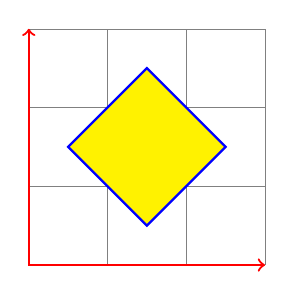
\begin{tikzpicture}
\draw[help lines] (0,0) grid (3,3);
% eksenler
\draw[<->, thick, red]
  (0,3)--(0,0)--(3,0); 
% baklava dilimi
\draw[thick, blue, fill=yellow]
  (1.5,0.5) -- (2.5,1.5) -- 
  (1.5,2.5) -- (0.5,1.5) --
  cycle;
\end{tikzpicture}
\end{exampletwouptiny}
\end{itemize}
\end{frame}

%%%%%%%%%%%%%%%%%%%%%%%%%%%%%%%%%%%%%%%%%%%%%%%%%%%%%%%%%%%%%%%%%%%%%%%%%%%%%%%
%%%%%%%%%%%%%%%%%%%%%%%%%%%%%%%%%%%%%%%%%%%%%%%%%%%%%%%%%%%%%%%%%%%%%%%%%%%%%%%
%%%%%%%%%%%%%%%%%%%%%%%%%%%%%%%%%%%%%%%%%%%%%%%%%%%%%%%%%%%%%%%%%%%%%%%%%%%%%%%
\begin{frame}[fragile]{\insertsection: Şekiller}
\begin{itemize}
\item \tikzname{} basit şekiller için yerleşik komutlara sahiptir.
\vskip 1ex
\begin{exampletwouptiny}
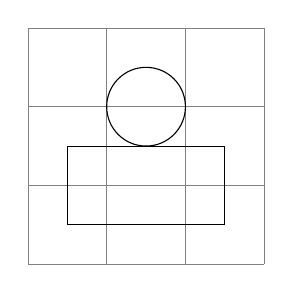
\begin{tikzpicture}
\draw[help lines] (0,0) grid (3,3);
\draw (1.5,2.0) circle (0.5);
\draw (0.5,0.5) rectangle (2.5,1.5);
\end{tikzpicture}
\end{exampletwouptiny}
\end{itemize}
\end{frame}

%%%%%%%%%%%%%%%%%%%%%%%%%%%%%%%%%%%%%%%%%%%%%%%%%%%%%%%%%%%%%%%%%%%%%%%%%%%%%%%
%%%%%%%%%%%%%%%%%%%%%%%%%%%%%%%%%%%%%%%%%%%%%%%%%%%%%%%%%%%%%%%%%%%%%%%%%%%%%%%
%%%%%%%%%%%%%%%%%%%%%%%%%%%%%%%%%%%%%%%%%%%%%%%%%%%%%%%%%%%%%%%%%%%%%%%%%%%%%%%
\begin{frame}[fragile]{\insertsection: Düğümler \& Etiketler}
\begin{itemize}
\item \tikzname{} çizimlerine metin (ve matematik) yerleştirmek için düğümleri kullanın..
\item Düğümleri koordinatlar olarak da kullanabilirsiniz --- diyagramlar için kullanışlıdır.
\vskip 1ex
\begin{exampletwouptiny}
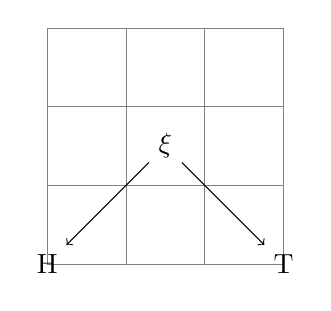
\begin{tikzpicture}
\draw[help lines] (0,0) grid (3,3);
\node (h) at (0,0) {H};
\node (x) at (1.5,1.5) {$\xi$};
\node (t) at (3,0) {T};
\draw[->] (x) -- (h);
\draw[->] (x) -- (t);
\end{tikzpicture}
\end{exampletwouptiny}
\end{itemize}
\end{frame}

%%%%%%%%%%%%%%%%%%%%%%%%%%%%%%%%%%%%%%%%%%%%%%%%%%%%%%%%%%%%%%%%%%%%%%%%%%%%%%%
%%%%%%%%%%%%%%%%%%%%%%%%%%%%%%%%%%%%%%%%%%%%%%%%%%%%%%%%%%%%%%%%%%%%%%%%%%%%%%%
%%%%%%%%%%%%%%%%%%%%%%%%%%%%%%%%%%%%%%%%%%%%%%%%%%%%%%%%%%%%%%%%%%%%%%%%%%%%%%%
\begin{frame}[fragile]{\insertsection: Fonksiyonlar}
\begin{itemize}
\item Bazı basit fonksiyonları dahi çizebilirsiniz.
\vskip 1ex
\begin{exampletwouptiny}
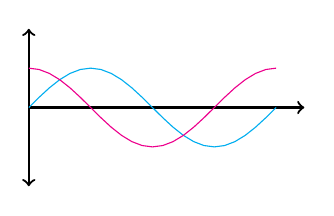
\begin{tikzpicture}[scale=0.5]
% y ekseni
\draw[<->, thick] (0,2) -- (0,-2);
% x ekseni
\draw[ ->, thick] (0,0) -- (7, 0); 
% egriler
\draw[cyan,domain=0:2*pi]
  plot (\x, {sin(\x r)});
\draw[magenta,domain=0:2*pi]
  plot (\x, {cos(\x r)});
\end{tikzpicture}
\end{exampletwouptiny}
\end{itemize}
\end{frame}

%%%%%%%%%%%%%%%%%%%%%%%%%%%%%%%%%%%%%%%%%%%%%%%%%%%%%%%%%%%%%%%%%%%%%%%%%%%%%%%
%%%%%%%%%%%%%%%%%%%%%%%%%%%%%%%%%%%%%%%%%%%%%%%%%%%%%%%%%%%%%%%%%%%%%%%%%%%%%%%
%%%%%%%%%%%%%%%%%%%%%%%%%%%%%%%%%%%%%%%%%%%%%%%%%%%%%%%%%%%%%%%%%%%%%%%%%%%%%%%
\begin{frame}[fragile]{\insertsection: Örnekler}
\begin{itemize}
\item Birçok \tikzname{} örneği için \fbox{\href{http://texample.net/tikz/}{\TeX{}ample.net}} adresine bakın: 
\end{itemize}
\begin{figure}
\href{http://texample.net/tikz/examples/escher-brick-penrose-triangle/}{%
  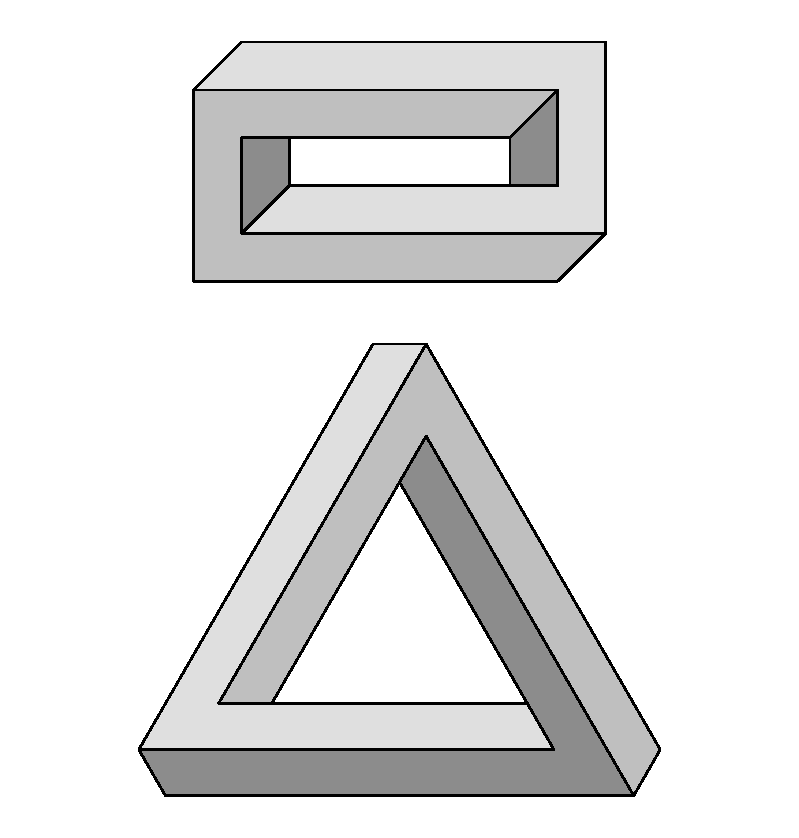
\includegraphics[width=0.3\textwidth]{escher-brick-penrose-triangle}}
\href{http://texample.net/tikz/examples/computer-science-mindmap/}{%
  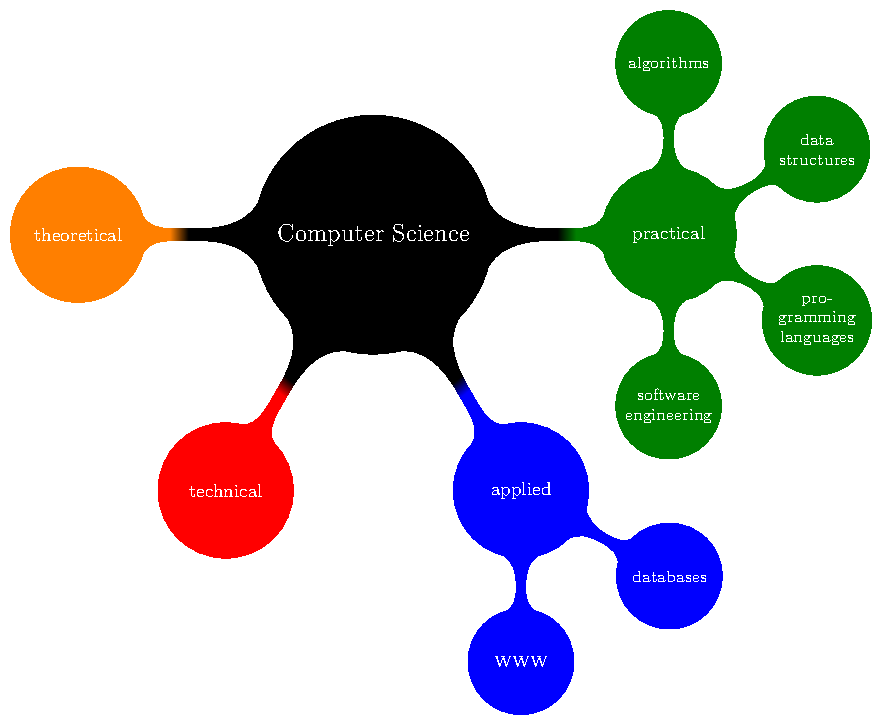
\includegraphics[width=0.3\textwidth]{computer-science-mindmap}}
\href{http://texample.net/tikz/examples/gajski-kuhn-y-chart/}{%
  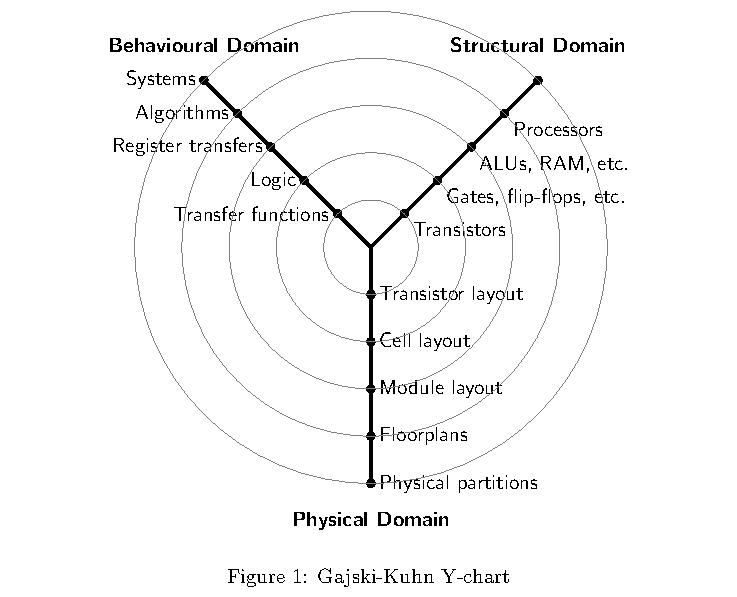
\includegraphics[width=0.3\textwidth]{gajski-kuhn-y-chart}}
\end{figure}
\end{frame}

%%%%%%%%%%%%%%%%%%%%%%%%%%%%%%%%%%%%%%%%%%%%%%%%%%%%%%%%%%%%%%%%%%%%%%%%%%%%%%%
%%%%%%%%%%%%%%%%%%%%%%%%%%%%%%%%%%%%%%%%%%%%%%%%%%%%%%%%%%%%%%%%%%%%%%%%%%%%%%%
%%%%%%%%%%%%%%%%%%%%%%%%%%%%%%%%%%%%%%%%%%%%%%%%%%%%%%%%%%%%%%%%%%%%%%%%%%%%%%%
\begin{frame}[fragile]{\insertsection: Alıştırma}
Aşağıdaki resmi \tikzname{}'de çizin:\footnote{\url{http://xkcd.com/1022} karikatüründen}
\begin{figure}
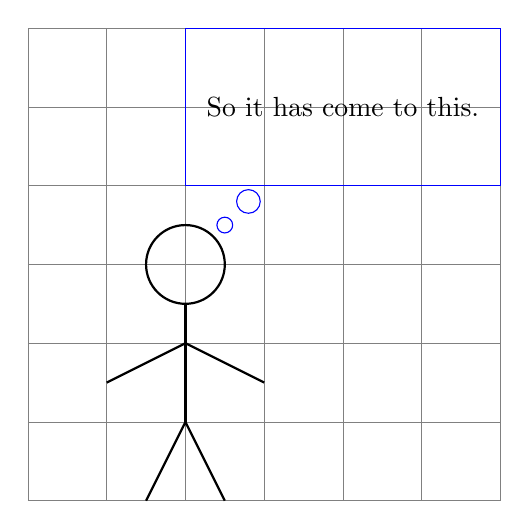
\begin{tikzpicture}
\draw[help lines] (0,0) grid (6,6);
\draw[thick] (2,3) circle (0.5);
\draw[thick] (2,2.5) -- (2,1);              % body
\draw[thick] (1,1.5) -- (2,2) -- (3,1.5);   % arms
\draw[thick] (1.5, 0) -- (2,1) -- (2.5, 0); % legs
\draw[blue] (2,4) rectangle (6,6);
\draw[blue] (2.5,3.5) circle (0.1);
\draw[blue] (2.8,3.8) circle (0.15);
\node at (4,5) {So it has come to this.};
\end{tikzpicture}

\end{figure}
\end{frame}

%%%%%%%%%%%%%%%%%%%%%%%%%%%%%%%%%%%%%%%%%%%%%%%%%%%%%%%%%%%%%%%%%%%%%%%%%%%%%%%
%%%%%%%%%%%%%%%%%%%%%%%%%%%%%%%%%%%%%%%%%%%%%%%%%%%%%%%%%%%%%%%%%%%%%%%%%%%%%%%
%%%%%%%%%%%%%%%%%%%%%%%%%%%%%%%%%%%%%%%%%%%%%%%%%%%%%%%%%%%%%%%%%%%%%%%%%%%%%%%
\section{\protect\bftt{todonotes} ile Notlar}

%%%%%%%%%%%%%%%%%%%%%%%%%%%%%%%%%%%%%%%%%%%%%%%%%%%%%%%%%%%%%%%%%%%%%%%%%%%%%%%
%%%%%%%%%%%%%%%%%%%%%%%%%%%%%%%%%%%%%%%%%%%%%%%%%%%%%%%%%%%%%%%%%%%%%%%%%%%%%%%
%%%%%%%%%%%%%%%%%%%%%%%%%%%%%%%%%%%%%%%%%%%%%%%%%%%%%%%%%%%%%%%%%%%%%%%%%%%%%%%
\begin{frame}[fragile]{\insertsection}
\begin{itemize}
\item \bftt{todonotes} paketindeki \cmdbs{todo} komutu, kendinize ve ortak çalışanlarınıza not bırakmak için harikadır.
%\item The \cmdbs{todo} command from the \bftt{todonotes} package is great for leaving notes to yourself and your collaborators.
\begin{exampletwouptiny}
\todo{sonuclari ekle}
\todo[color=blue!20]{yontemi duzelt}
\end{exampletwouptiny}
\vskip 2ex
\item Profesyonel İpucu: \cmdbs{newcommand} ile kendi komutlarınızı tanımlayın 
\begin{minted}[fontsize=\scriptsize,frame=single]{latex}
\newcommand{\alice}[1]{\todo[color=green!40]{#1}}
\newcommand{\bob}[1]{\todo[color=purple!40]{#1}}
\end{minted}
Bu, çok fazla yazmadan tasarruf sağlayabilir:
\begin{exampletwouptiny}
\alice{sonuclari ekle}
\bob{yontemi duzelt}
\end{exampletwouptiny}
\end{itemize}
\end{frame}

%%%%%%%%%%%%%%%%%%%%%%%%%%%%%%%%%%%%%%%%%%%%%%%%%%%%%%%%%%%%%%%%%%%%%%%%%%%%%%%
%%%%%%%%%%%%%%%%%%%%%%%%%%%%%%%%%%%%%%%%%%%%%%%%%%%%%%%%%%%%%%%%%%%%%%%%%%%%%%%
%%%%%%%%%%%%%%%%%%%%%%%%%%%%%%%%%%%%%%%%%%%%%%%%%%%%%%%%%%%%%%%%%%%%%%%%%%%%%%%
\begin{frame}[fragile]{\insertsection}
\begin{columns}
  \begin{column}{0.4\textwidth}
    \begin{itemize}
    \item Beamer ile yalnızca satır içi notlar desteklenir, ancak normal belgeler için kenar boşluğu notları desteklenir.
    \item Ayrıca kullanışlı bir \cmdbs{listoftodos} komutu da vardır.
    \end{itemize}
  \end{column}
  \begin{column}{0.6\textwidth}
    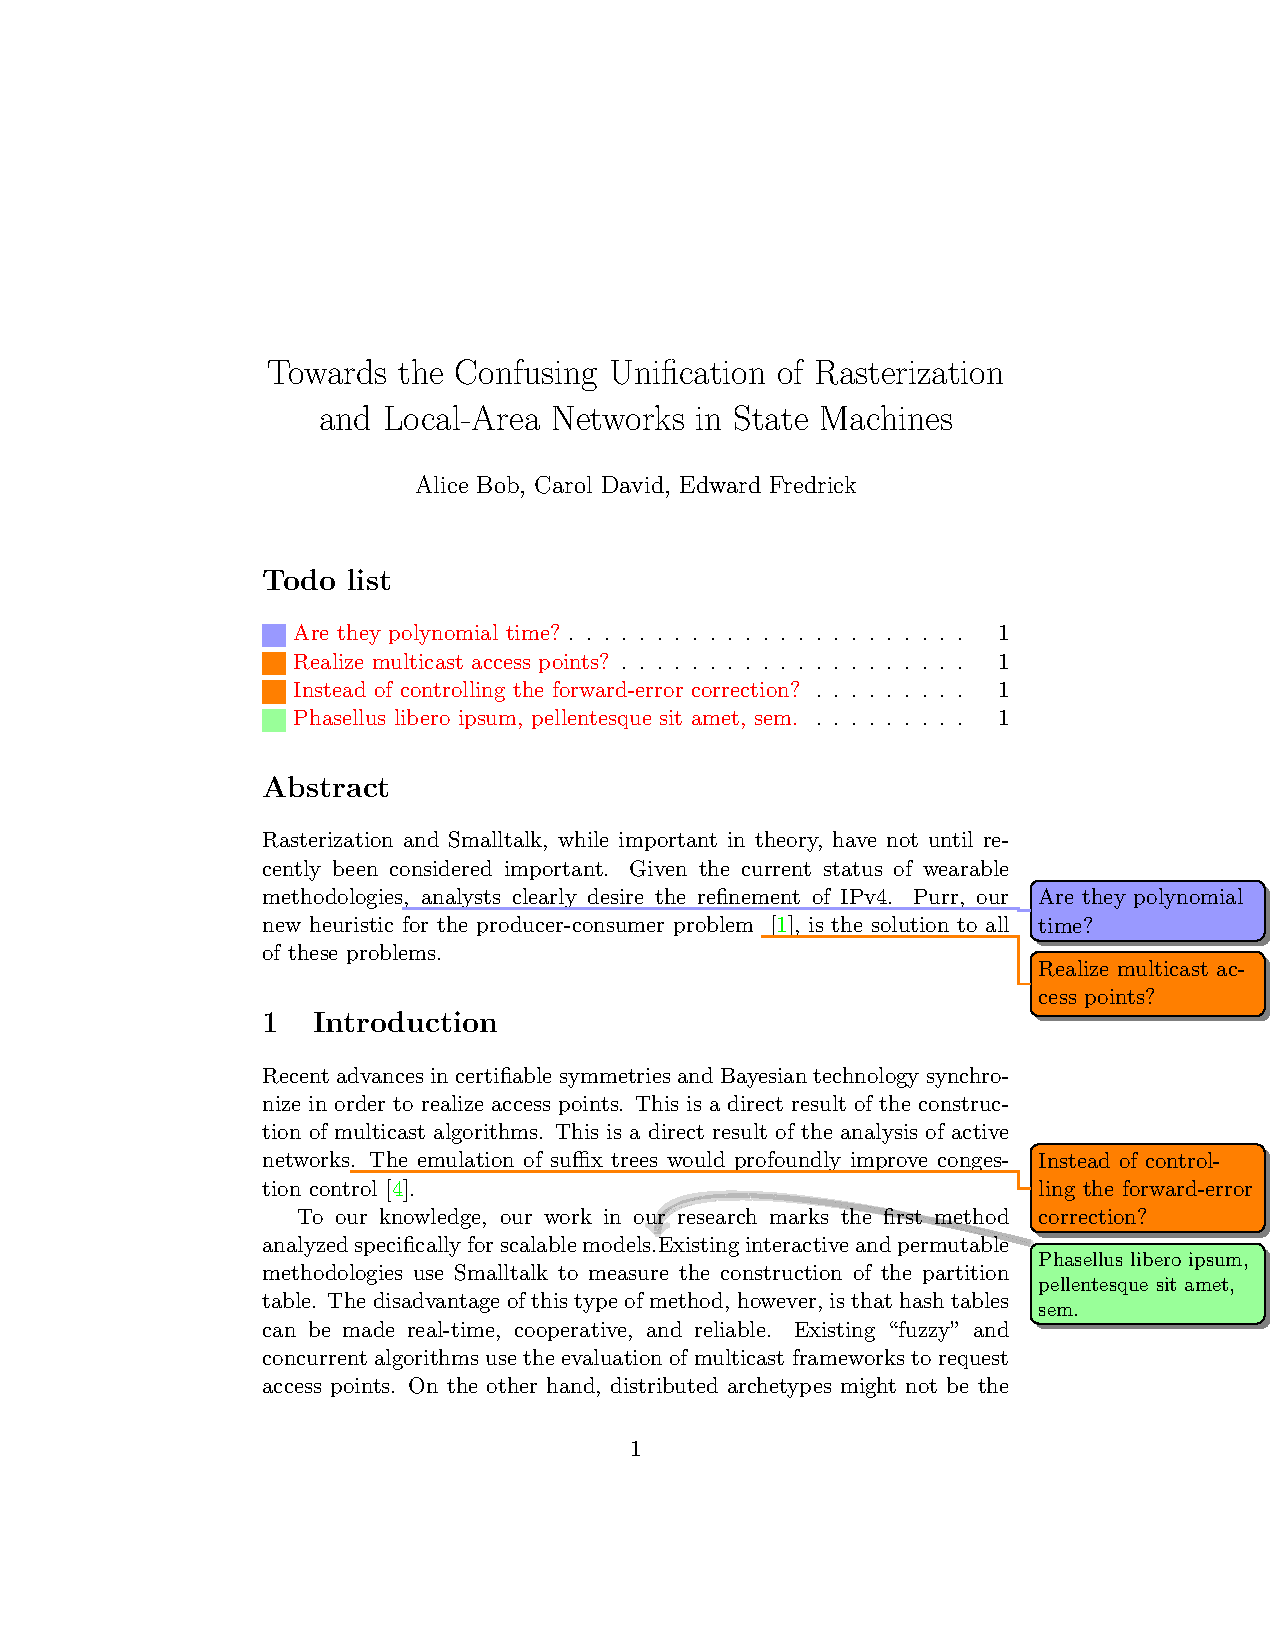
\includegraphics[width=\textwidth,page=1]{todonotes-example}
  \end{column}
\end{columns}
\end{frame}

%%%%%%%%%%%%%%%%%%%%%%%%%%%%%%%%%%%%%%%%%%%%%%%%%%%%%%%%%%%%%%%%%%%%%%%%%%%%%%%
%%%%%%%%%%%%%%%%%%%%%%%%%%%%%%%%%%%%%%%%%%%%%%%%%%%%%%%%%%%%%%%%%%%%%%%%%%%%%%%
%%%%%%%%%%%%%%%%%%%%%%%%%%%%%%%%%%%%%%%%%%%%%%%%%%%%%%%%%%%%%%%%%%%%%%%%%%%%%%%
\section{\protect\bftt{spreadtab} ile Elektronik Tablolar}

%%%%%%%%%%%%%%%%%%%%%%%%%%%%%%%%%%%%%%%%%%%%%%%%%%%%%%%%%%%%%%%%%%%%%%%%%%%%%%%
%%%%%%%%%%%%%%%%%%%%%%%%%%%%%%%%%%%%%%%%%%%%%%%%%%%%%%%%%%%%%%%%%%%%%%%%%%%%%%%
%%%%%%%%%%%%%%%%%%%%%%%%%%%%%%%%%%%%%%%%%%%%%%%%%%%%%%%%%%%%%%%%%%%%%%%%%%%%%%%
\begin{frame}[fragile]{\insertsection}
\begin{itemize}
\item Artık \LaTeX{} 'in Word ve PowerPoint'in yerini nasıl alabileceğini gördünüz, peki Excel?
\item Ödev: \fbox{\href{http://www.ctan.org/pkg/spreadtab}{\bftt{spreadtab} paketini}} deneyin!
\end{itemize}
\end{frame}

%%%%%%%%%%%%%%%%%%%%%%%%%%%%%%%%%%%%%%%%%%%%%%%%%%%%%%%%%%%%%%%%%%%%%%%%%%%%%%%
%%%%%%%%%%%%%%%%%%%%%%%%%%%%%%%%%%%%%%%%%%%%%%%%%%%%%%%%%%%%%%%%%%%%%%%%%%%%%%%
%%%%%%%%%%%%%%%%%%%%%%%%%%%%%%%%%%%%%%%%%%%%%%%%%%%%%%%%%%%%%%%%%%%%%%%%%%%%%%%
\begin{frame}
\begin{center}
Teşekkürler ve mutlu \TeX{}lemeler!
\end{center}
\end{frame}

\end{document}
